% Load Useful Packages
\documentclass[12pt]{beamer}
\usepackage[utf8]{inputenc}
\usepackage{graphicx}
\usepackage{tikz}
\usepackage{aeguill}
\usepackage{minted}
%\input{defaults}
\usepackage{bm}
\usepackage{amsmath}
\usepackage{amsfonts}
\usepackage{amssymb}
\usepackage{hyperref}

% Define Theme
% Oxford Blue is RGB={0,33,71}
% \usefonttheme{structuresmallcapsserif} 
\usetheme{Rochester}
\usecolortheme[RGB={0,33,71}]{structure}
\setbeamertemplate{navigation symbols}{}
\setbeamertemplate{items}[circle]

% Title Information
\author[C. MacMackin]{Christopher MacMackin}
\title{Writing Scientific Software}
\subtitle{Lessons from the Software Engineering Community}
\date[Nov. 2016]{4 November 2016}
\institute[Oxford]{Atmospheric, Oceanic, and Planetary Physics \\
  University of Oxford \\
  Oxford, UK \\[1ex]
  christopher.macmackin@physics.ox.ac.uk\\
  cmacmackin.github.io
}

\begin{document}
% Title Slide
\begin{frame}[plain]
  \titlepage
\end{frame}

% General Presentation
\section*{Managing Large Codes}
\begin{frame}
  \frametitle{Glaciologist by day\ldots}
  \begin{center}
    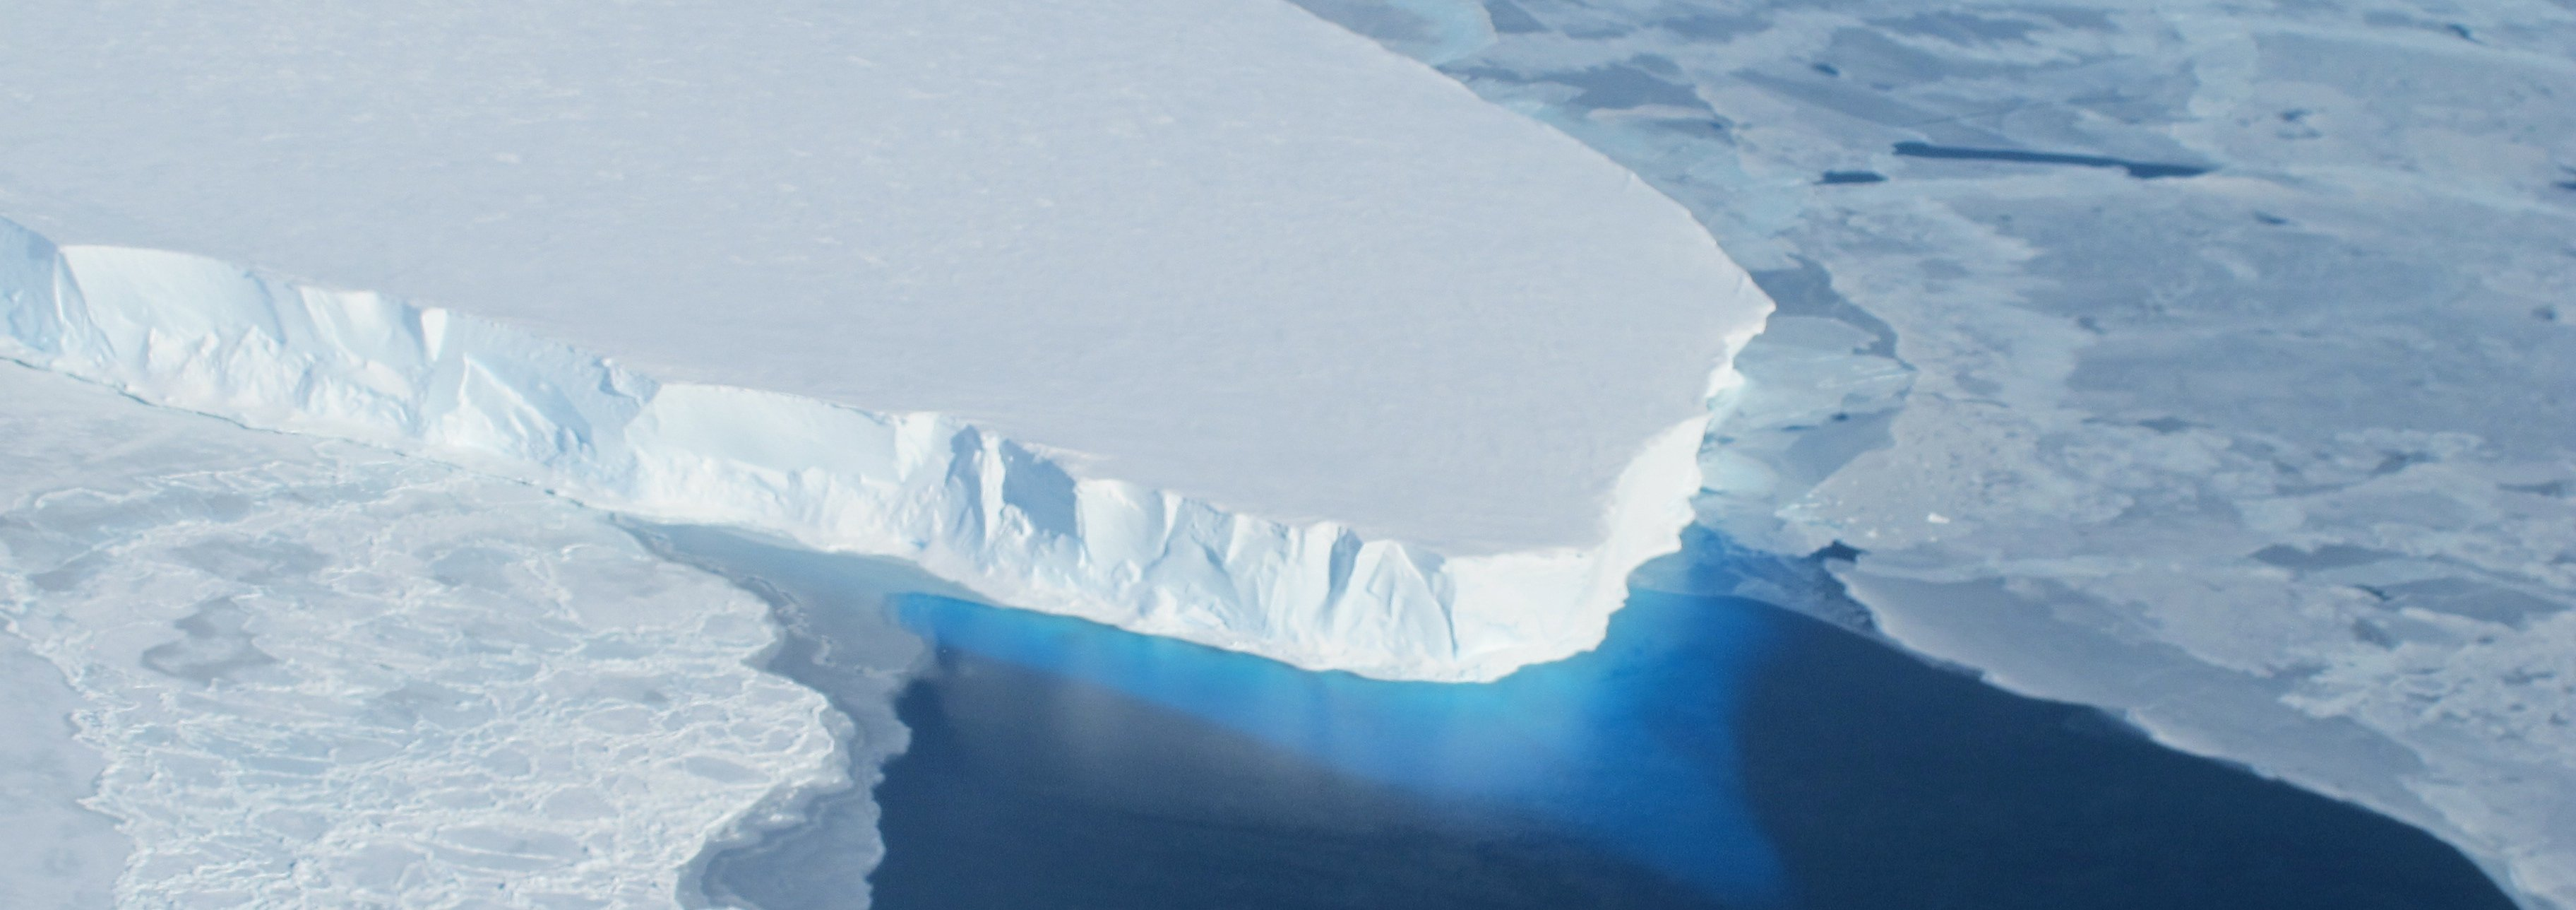
\includegraphics[width=0.9\textwidth]{shelfPhoto.jpg}
    
    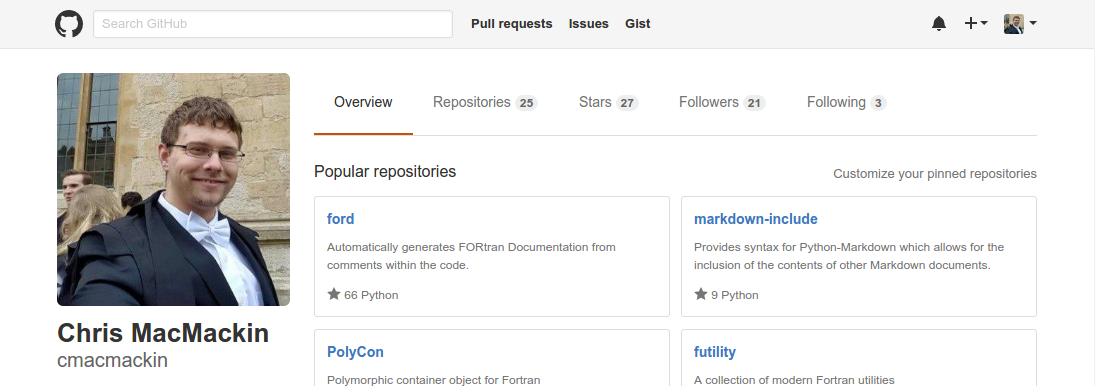
\includegraphics[width=0.9\textwidth]{github.png}
  \end{center}

\end{frame}

\begin{frame}{Scientists are not Programmers}
  Problem:
  \begin{itemize}
  \item Science relies on increasingly large codes
  \item Large codes become complex, difficult to maintain
  \item Improving or altering codes becomes more time consuming
  \end{itemize}
  
  \vspace{2mm}
  These problems can be mitigated by good design. \textbf{But,}
  \begin{itemize}
  \item Scientists not taught software design
  \item Code often written quickly, is unmaintainable
  \item Can end up costing more time in the long run
  \end{itemize}
\end{frame}

\begin{frame}
  \frametitle{(Real) Example}
  A magneto-hydrodynamics code:
  \begin{itemize}
  \item 130 thousand lines long
  \item All in one file
  \item No procedure has name longer than 8 characters
  \item All important variables global
  \end{itemize}
  
  Only maintainable if you have worked with it for years.
  
  \begin{center}
    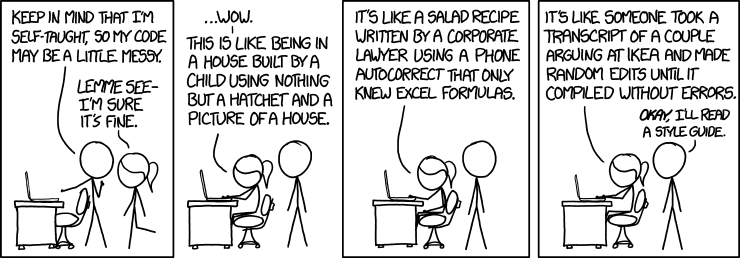
\includegraphics[width=0.9\textwidth]{code_quality.png}
    
    \vspace{-2mm}{\tiny https://xkcd.com/1513/}
  \end{center}
  
\end{frame}

% Table of Contents
\begin{frame}{Outline}
  \tableofcontents
\end{frame}


% Introduce object-oriented programming design with UML
\section{Modern Programming Paradigms}

% Quick overview of object oriented programming
\subsection{Object Oriented Programming}

\begin{frame}
  \frametitle{Object Oriented Programming}
  OOP is now the dominant programming paradigm.
  % software.
  \begin{itemize}
  \item Define ``classes'', like new data-types
  \item Classes contain data, have associated procedures
  \item Variables of these types are ``objects''
  \end{itemize}
  
  \vspace{3mm}
  Object oriented languages feature:
  
  \begin{description}
  \item[Encapsulation] controlling what data can be seen by different
    procedures
  \item[Inheritance] ``Is-a-type-of'' relationship, giving subclasses
    access to parent's methods 
  \item[Polymorphism] Ability to run code without knowing exact type
    of an object
  \end{description}
\end{frame}

% \begin{frame}[fragile=singleslide]
%   \frametitle{Example in Fortran}
%   \begin{minted}[gobble=4]{fortran}
%     type :: person
%     real                          :: weight
%     character(len=:), allocatable :: name
%     contains
%     procedure :: die
%     procedure :: pay_taxes
%     end type person
%     
%     type, extends(person) :: employee
%     real :: salary
%     contains
%     procedure :: pay_taxes
%     procedure :: collect_salary
%     end type 
%   \end{minted}
% \end{frame}

\begin{frame}
  \frametitle{Why OOP?}
  Object oriented programming has following advantages:
  \begin{itemize}
  \item Useful way to organise data
  \item Can use one object as argument, rather than many
  \item Increases code-reuse via inheritance
  \item Conceptually convenient way to partition code
  \item Define an interface, independent of implementation
  \end{itemize}

  \vspace{3mm}
  However (e.g. arithmetic), some things best accomplished
  through other paradigms.
\end{frame}

% Introduce this principle, explaining why
\subsection{Interfaces, not Implementations}

\begin{frame}
  \frametitle{Program to an Interface}
  Changing one part of the code, shouldn't force you to change
  other parts. Can do this is by defining an API.
  
  \begin{definition}
    \structure{API}: Application Programming Interface 
  \end{definition}
  
  \begin{enumerate}
  \item Create procedures stubs provide desired functionality
  \item Prevent direct access to any non-constant variables
  \item Write procedure bodies
  \item If making changes, don't alter names, arguments, return values
    of publicly accessible procedures
  \end{enumerate}
\end{frame}

\begin{frame}
  \frametitle{But I Really Need to Change It!}
  Would you like it if a new version of PETSc changed so it no longer
  worked with your code?
  
  \vspace{3mm}
  Strategies:
  \begin{itemize}
  \item Add optional arguments
  \item Add new procedures, overload old ones
  \item Design it well in the first place
  \end{itemize}
  
  \vspace{2mm}
  \begin{center}
    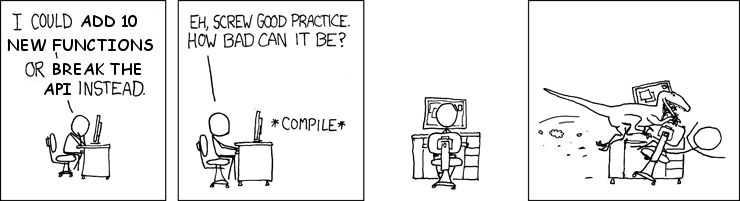
\includegraphics[width=0.95\textwidth]{break_api.png}
    
    \vspace{-2mm}{\scriptsize (With apologies to Randall Munroe.)}
    {\tiny https://xkcd.com/292/}
  \end{center}

\end{frame}

% Introduction to UML
\subsection{Unified Modelling Language}

\begin{frame}
  \frametitle{Describing Your Software}
  When designing code, can be useful to have way to easily represent
  its structure, relationships.
  
  % \begin{center}
  %   
\includegraphics[height=0.28\textheight]{uml_logo.png}
  % \end{center}
  
  \vspace{3mm}
  \textit{Unified Modelling Language} (UML): standardised
  collection of graphical elements to do that.% Programming language
  % agnostic, can produce various types of diagrams.
  
  \vspace{3mm}
  Examples of free software to produce UML:
  
  \begin{columns}
    \begin{column}{0.5\textwidth}
      \centering
      
\includegraphics[height=0.2\textheight]{dia.png}
      
      Dia (GUI)
    \end{column}
    \begin{column}{0.5\textwidth}
      \centering
      
\includegraphics[height=0.2\textheight]{plantuml.png}
      
      PlantUML (language)
    \end{column}
  \end{columns}
  
  \vspace{3mm}
  Will use UML in this presentation. (Pay attention!)
\end{frame}

\begin{frame}
  \frametitle{UML Class Diagrams}
  Can describe contents of a class/derived type:
  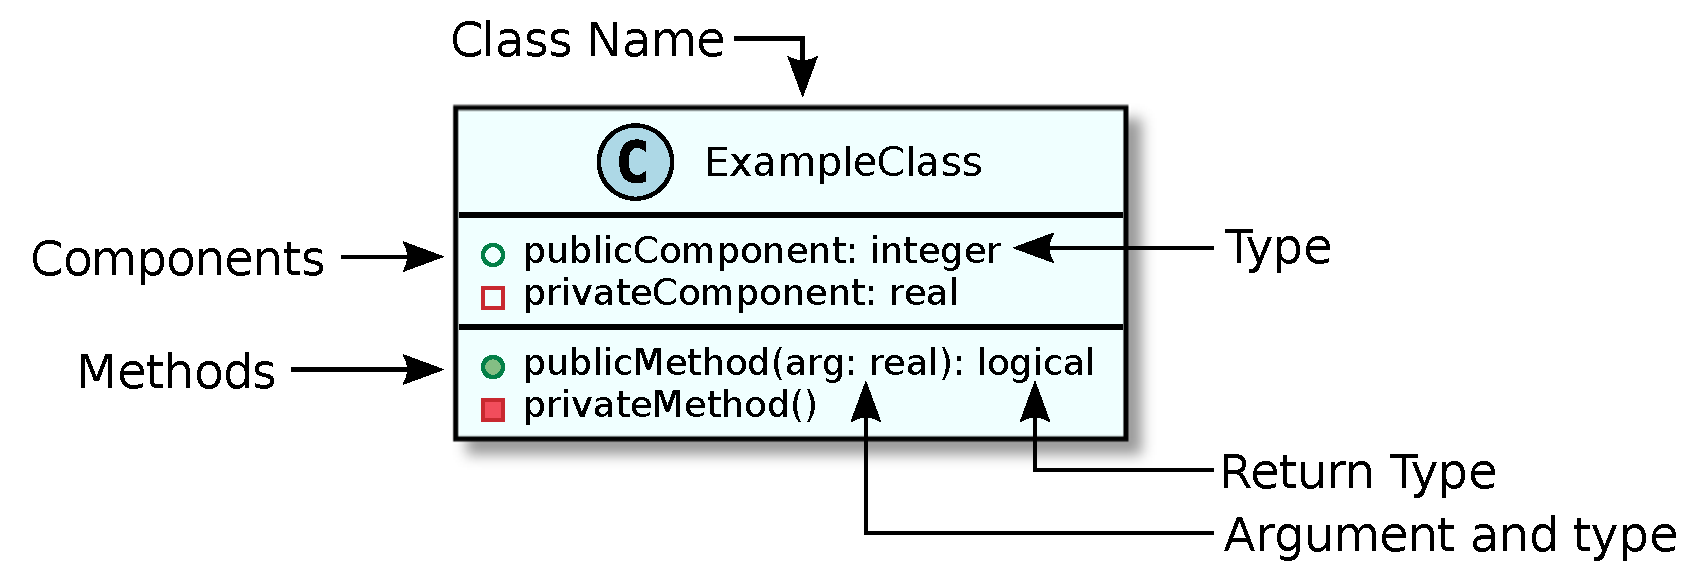
\includegraphics[width=\textwidth]{class_diagram.pdf}
  % 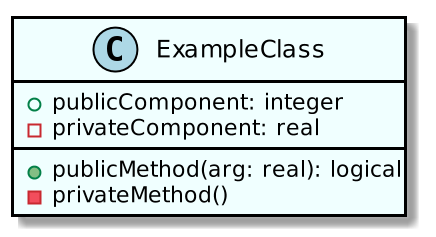
\includegraphics[width=0.5\textwidth]{class_diagram.png}
  
  \begin{columns}
    \begin{column}{0.55\textwidth}
      Note that \texttt{public}/\texttt{private} also specified with
      ``+''/``-'':
    \end{column}
    \begin{column}{0.45\textwidth}
      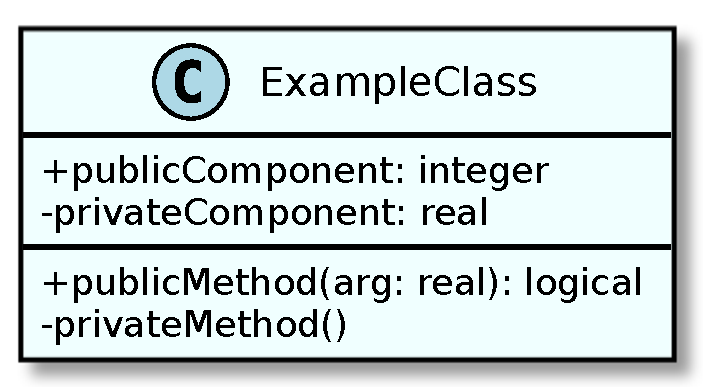
\includegraphics[width=\textwidth]{class_diagram_plain.pdf}
    \end{column}
  \end{columns}
\end{frame}

\begin{frame}
  \frametitle{UML Class Relationships}
  Can also show how classes inherit from or contain others.
  
  \vspace{3mm}
  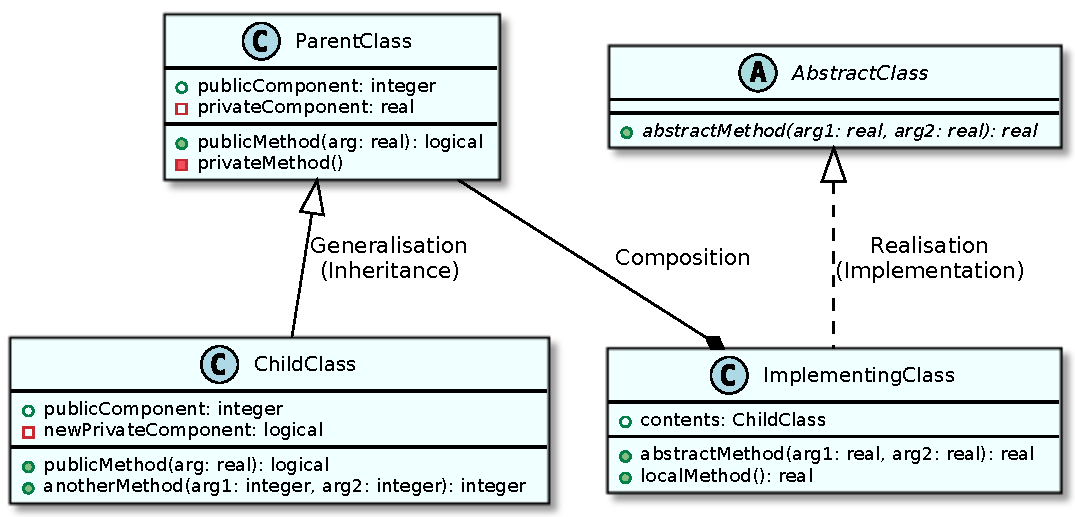
\includegraphics[width=\textwidth]{inheritance_diagram.pdf}
\end{frame}

\begin{frame}
  \frametitle{UML Sequence Diagrams}
  UML diagrams can also describe call sequence.
  
  \begin{center}
    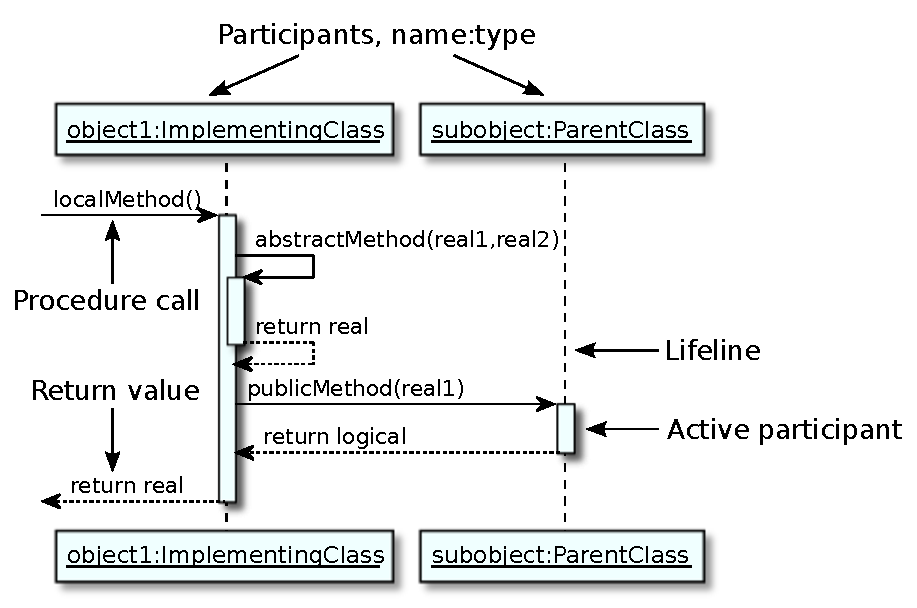
\includegraphics[width=0.93\textwidth]{sequence_diagram.pdf}
  \end{center}

\end{frame}


% % Discuss various software etc. to make your life easier
% \section{Programming Tools}

% \begin{frame}
%   \frametitle{Development Cycle}
%   Software development (roughly) consists of following steps:
%   \begin{enumerate}
%   \item Analysis: Consider the problem at hand
%   \item Design: Choose algorithms and structures to use in software
%   \item Implementation: Write the code
%   \item Testing: Check that the code does what it should
%   \item Deployment: Make the code ready for use by others
%   \item Maintenance: Use the code in production, ensure it continues working
%   \end{enumerate}
%   Tools exist which can help with each step
% \end{frame}

% % Talk about git and GitHub
% % \subsection{Version Control}

% % Benefits/techniques of unit testing, mention pFUnit
% \subsection{Unit Testing}
% \begin{frame}
%   \frametitle{Ensuring it Works}

% \end{frame}

% \begin{frame}
%   \frametitle{Assertions}

% \end{frame}

% \begin{frame}
%   \frametitle{Unit Test Frameworks}

% \end{frame}

% % Explain benefits of documentation, quickly demonstrate FORD
% \subsection{Automatic Documentation}

% \begin{frame}
%   \frametitle{What Does this Do?}

% \end{frame}

% \begin{frame}
%   \frametitle{Automatic Documentation}

% \end{frame}

% \begin{frame}
%   \frametitle{Example}

% \end{frame}


% Explain the design patterns introduced by Rouson et al.
\section{Design Patterns for Scientific Code}

\begin{frame}
  \frametitle{Design Patterns}
  \begin{columns}
    \begin{column}{0.5\textwidth}
      Writing software, common problems frequently reoccur. 
      Canonical solutions have been developed called \textit{design
        patterns}.
      
      \vspace{3mm} Many general-purpose patterns can be relevant
      to scientific software. Will focus here on domain-specific
      patterns introduced by Rouson, Xia, and Xu (2011).
    \end{column}
    \begin{column}{0.5\textwidth}
      \begin{center}
        
\includegraphics[height=0.9\textheight]{Rouson.jpg}
      \end{center}

    \end{column}
  \end{columns}
\end{frame}

% Explain what this patter does and give a simple example
\subsection{The Abstract Calculus Pattern}

\begin{frame}
  \frametitle{The Abstract Calculus Pattern}
  \begin{block}{The Problem}
    Physics and mathematics use high level representations of concepts
    which can not be simply expressed in code.
  \end{block}

  \vspace{2mm}
  Consider integration using the forward Euler
  method,
  $$ T(x,t+\Delta t) = T(x,t) + \Delta t\frac{\partial T(x,t)}{\partial
    t}. $$
  But code will look quite different and much messier than this. Also
  somewhat difficult to reuse. (Even worse for coupled equations.)
\end{frame}

\begin{frame}[fragile=singleslide]
  \frametitle{Abstract Calculus to the Rescue!}
  \begin{columns}
    \begin{column}{0.5\textwidth}
      We can take advantage of operator overloading to provide a nice
      syntax:
    \end{column}
    \begin{column}{0.5\textwidth}
      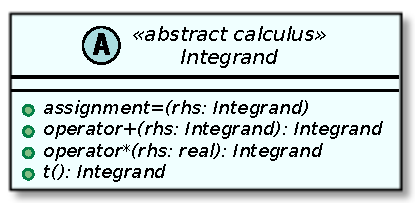
\includegraphics[width=\textwidth]{abstract_calculus.pdf}
    \end{column}
  \end{columns}
  
  \vspace{3mm}
  \begin{minted}[gobble=4,mathescape]{fortran}
    subroutine integrate(T, dt)
    class(integrand), intent(inout) :: T
    real, intent(in) :: dt
    ! Forward Euler integration:
    ! $T^{n+1}=T^{n}+T_t{\Delta}t$
    T = T + T%t()*dt
    end subroutine integrate
  \end{minted}
\end{frame}

\begin{frame}
  \frametitle{The Why and Wherefore}
  Using an abstract \texttt{integrand} type facilitates reuse of
  integration code, which is agnostic towards:
  
  \begin{itemize}
  \item Type of problem
  \item Storage pattern of data
  \item Precision of data
  \item Size of computational domain
  \end{itemize}
  
  Elegance of syntax useful for higher-order methods. Can also apply
  pattern to, e.g., vector calculus:
  $$ \bm{g} = -\nabla\phi \quad \rightarrow \quad \mathtt{g = -\
    .grad.\ phi} $$
\end{frame}

% Describe how this handles interactions and why that is a good thing
\subsection{The Puppeteer Pattern}

\begin{frame}
  \frametitle{The Puppeteer Pattern}
  \begin{columns}
    \begin{column}{0.55\textwidth}
      Often it is impractical to package entire program together. E.g.,
      ``multiphysics'' problems have many components.
      
      \vspace{3mm} $N$ components $\Rightarrow N(N+1)$
      interdependencies.

      \vspace{3mm}Complexity/fragility grows quickly. Also
      becomes harder to maintain data-hiding.
    \end{column}
    \begin{column}{0.45\textwidth}
      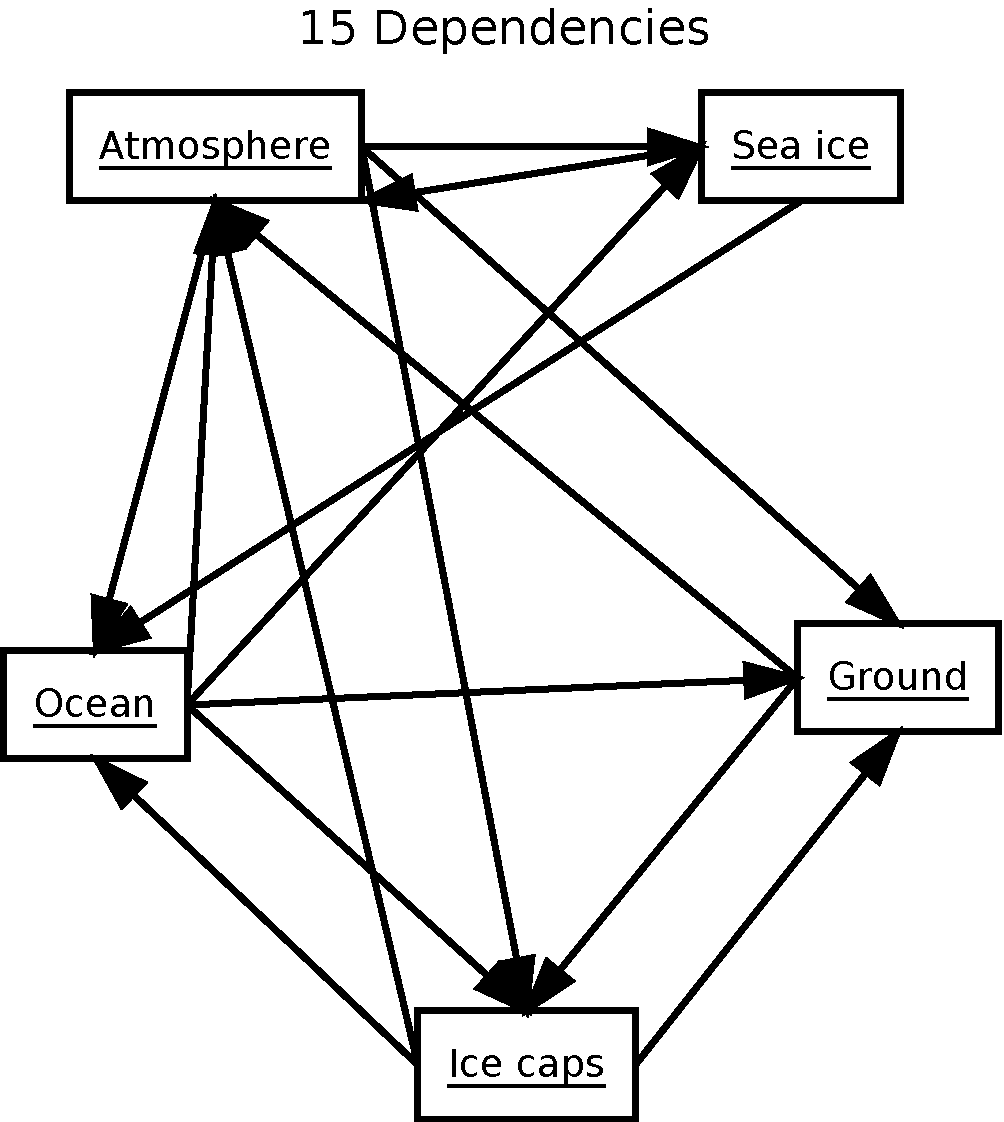
\includegraphics[width=\textwidth]{dependencies.pdf}
    \end{column}
  \end{columns}
\end{frame}

\begin{frame}
  \frametitle{Puppeteers to the Rescue!}
  \begin{columns}
    \begin{column}{0.55\textwidth}
      Can use a single class to manage interactions between all
      others. Only the one class needs to know the interfaces of the
      others.
      \begin{center}
        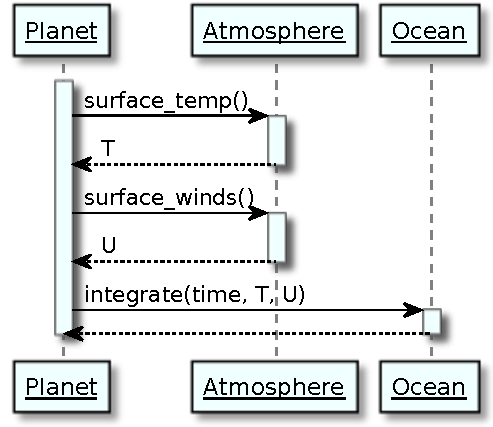
\includegraphics[width=0.9\textwidth]{puppeteer_sequence.pdf}
      \end{center}
    \end{column}
    \begin{column}{0.45\textwidth}
      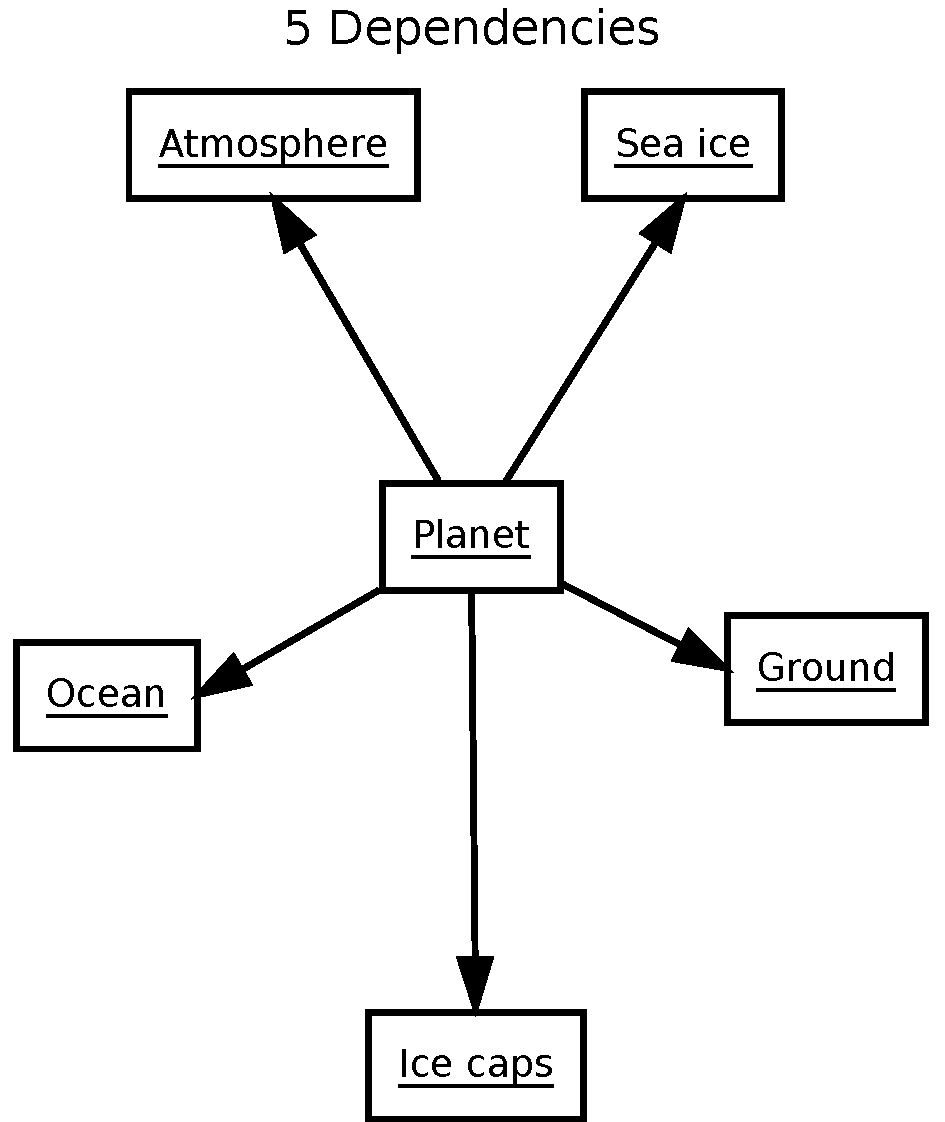
\includegraphics[width=\textwidth]{puppeteer_deps.pdf}
    \end{column}
  \end{columns}
\end{frame}

\begin{frame}
  \frametitle{The Why and Wherefore}
  This provides many advantages:
  \begin{itemize}
  \item Changing component's API affects only  puppeteer 
  \item Avoids circular dependencies
  \item Each component designed independently from others
  \item Can easily turn components off, decoupling system
  \item Place to assemble global data (e.g.\ a Jacobian)
  \end{itemize}

  \vspace{3mm}
  A puppeteer may be a concrete implementation of abstract calculus.
\end{frame}


% Go into ISOFT/FACTUAL to provide examples of this
\section{Case Study: Ice Shelf Model}

\begin{frame}
  \frametitle{Case Study: Ice Shelf}
  \begin{center}
    \setlength{\fboxsep}{0pt}
    \setlength{\fboxrule}{0.5pt}
    \fbox{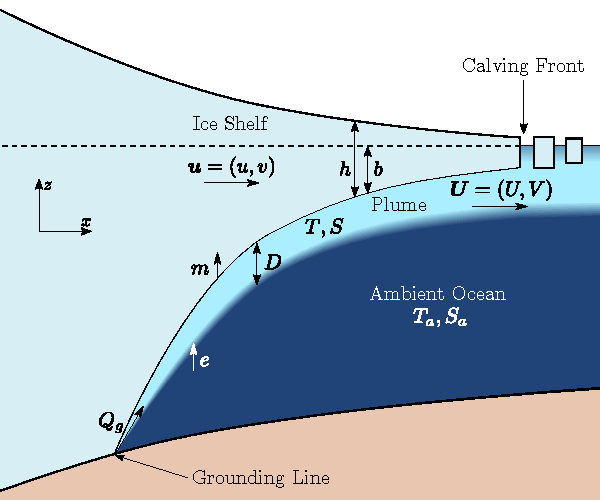
\includegraphics[height=0.92\textheight]{iceshelf.pdf}}
  \end{center}
\end{frame}

\begin{frame}
  \frametitle{Equations}
  \structure{Ice Shelf}
  $$ h_{t} + \nabla\cdot(h\vec{u}) = -\lambda m, $$
  $$ {\left(4\eta hu_x\right)}_{x} - \chi{\left(h^2\right)}_x = 0. $$
  
  \structure{Plume}
  $$ \nabla\cdot\left(D\vec{U}\right) = e + m, $$
  \begin{multline*}
    \nabla\cdot\left(D\vec{U}U\right) = D(\rho_a - \rho)\left(b_x -
      \delta D_x\right) + \nu\nabla\cdot\left(D\nabla U\right) \\
    - \mu|\vec{U}|U + \frac{\delta D^2}{2}\rho_x,
  \end{multline*}
  $$ \nabla\cdot\left(D\vec{U}S\right) = eS_a
  + \nu\nabla\cdot\left(D\nabla S\right) + mS_m - \gamma_S(S-S_m), $$
  $$ \nabla\cdot\left(D\vec{U}T\right) = eT_a
  + \nu\nabla\cdot\left(D\nabla T\right) + mT_m - \gamma_T(T-T_m). $$
\end{frame}

% Show hierarchy of puppeteers and the field type
\begin{frame}
  \frametitle{Breaking Down the Problem}
  Choice of numerics:
  \begin{itemize}
  \item Chebyshev pseudo-spectral spatial discretisation
  \item Backwards-Euler time integration
  \end{itemize}
  
  \vspace{3mm}
  Let $S(t)$ be state of ice shelf at time $t$, with
  $\dot{S}(S,m)$. The melt rate is $m(S,t)$. Backwards-Euler requres
  $$ S(t+\Delta t) = S(t) + \dot{S}[S(t+\Delta t),m]\Delta t. $$
  
  This requires iterative nonlinear solver. To reduce cost of this,
  evaluate $m[S(t),t]$---semi-implicit method.
\end{frame}

\begin{frame}
  \frametitle{Collating our Classes}
  \begin{center}
    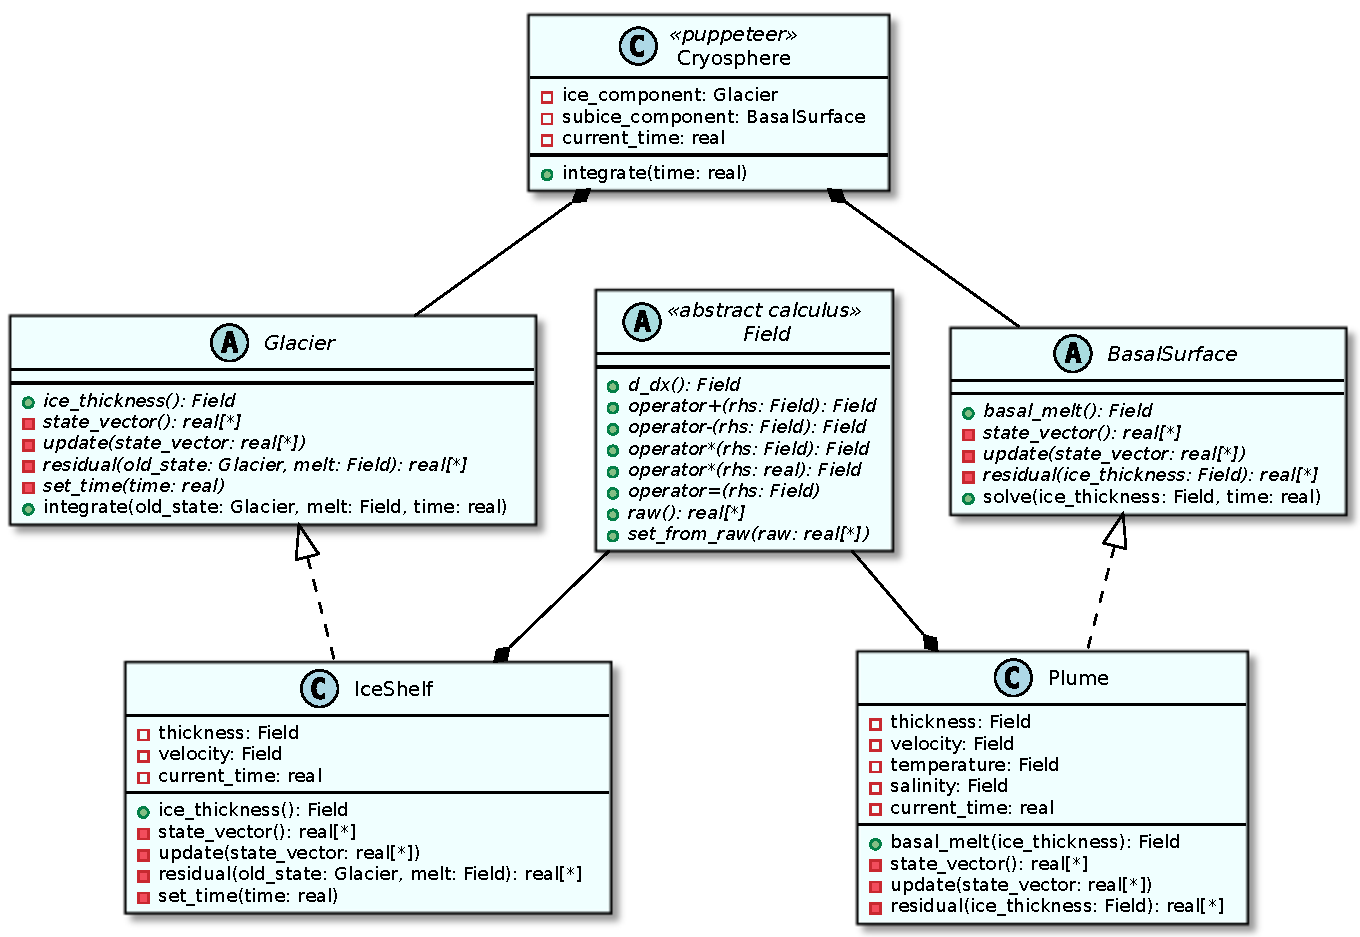
\includegraphics[width=0.95\textwidth]{isoft_classes.pdf}
  \end{center}
\end{frame}

\begin{frame}
  \frametitle{Solution Sequence}
  \begin{center}
    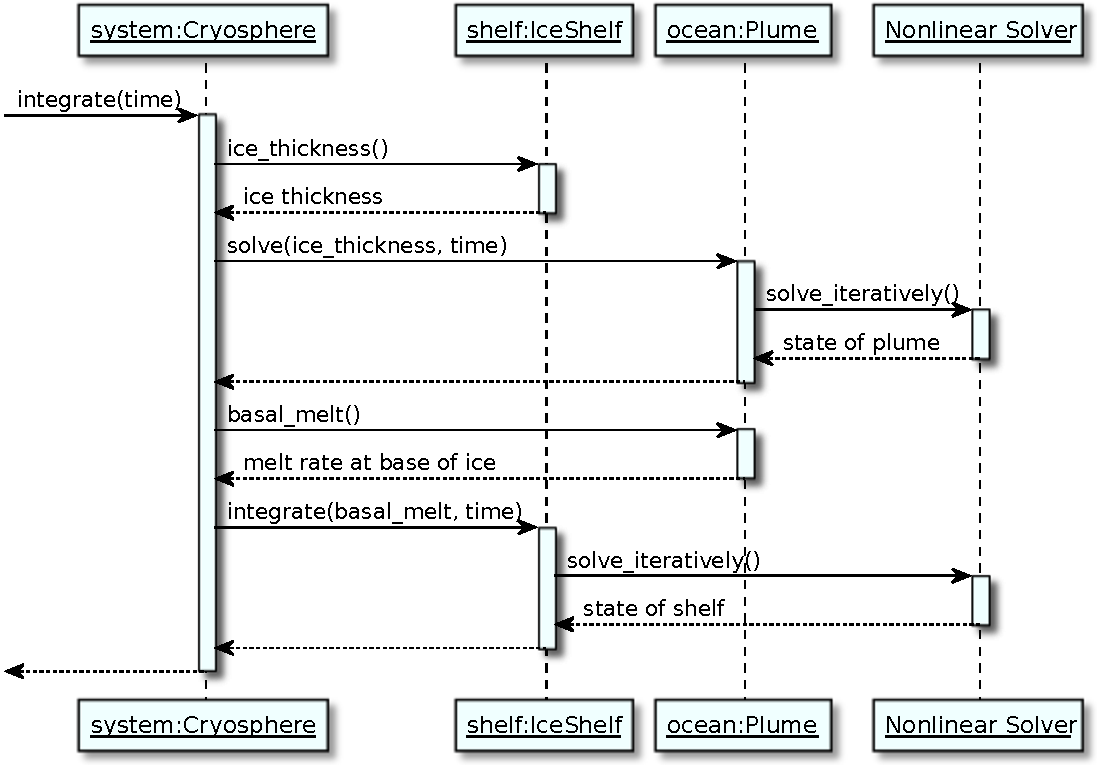
\includegraphics[width=0.95\textwidth]{isoft_sequence.pdf}
  \end{center}
\end{frame}

% Demonstrate how using abstract types make it easy to change parameterisations
\begin{frame}
  \frametitle{Parameterisation Choices}
  Will be useful to compare results for different parameterisations
  of, e.g.:
  \begin{itemize}
  \item viscosity
  \item melting
  \item entrainment
  \end{itemize}
  
  To make it easy to switch these, use the ``strategy'' pattern.
  \begin{center}
    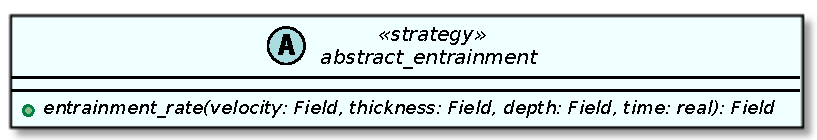
\includegraphics[width=\textwidth]{parameterisations.pdf}
  \end{center}
\end{frame}


% Conclusion
\section{Conclusion}

\begin{frame}
  \frametitle{Is it worth it?}
  \begin{center}
    \textit{``I find that when someone's taking time to do something
      right in the present, they're a perfectionist with no ability to
      prioritize, whereas when someone took time to do something right
      in the past, they're a master artisan of great foresight.''}
    
    \vspace{5mm}
    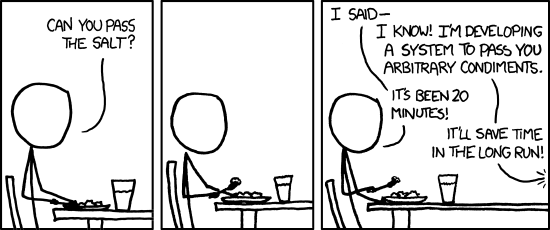
\includegraphics[width=0.8\textwidth]{the_general_problem.png}
    
    {\tiny https://xkcd.com/974/}
  \end{center}
\end{frame}

\begin{frame}{Summary}
  \begin{columns}
    \begin{column}{0.6\textwidth}
      Science is increasingly reliant on large pieces of
      software.
      
      \begin{itemize}
      \item Think before coding!
      \item Plan your software (e.g.\ with UML)
      \item Program to an interface
      \item Leverage language features for natural syntax
      \item Minimise inter-dependency
      \end{itemize}
      
      Time invested up front \textit{can} save time later.
    \end{column}
    \begin{column}{0.4\textwidth}
      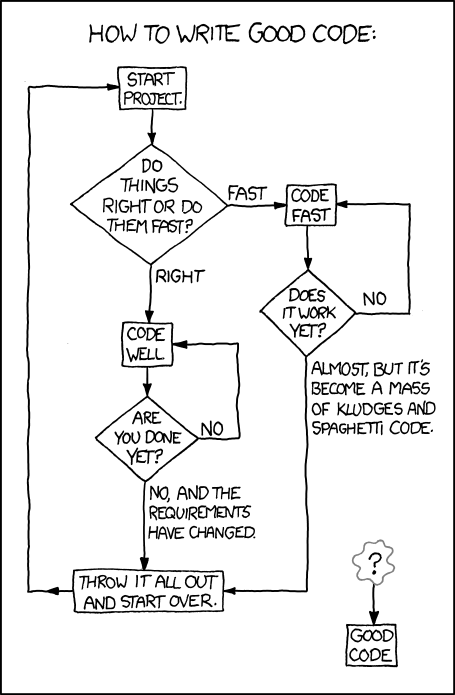
\includegraphics[width=\textwidth]{good_code.png}

      \vspace{-3mm}
      {\tiny https://xkcd.com/844/}
    \end{column}
  \end{columns}
\end{frame}

\begin{frame}{Thank You}
  \begin{center}
    \structure{\Huge Questions?}
  \end{center}
\end{frame}

\begin{frame}[plain]
  \begin{center}
    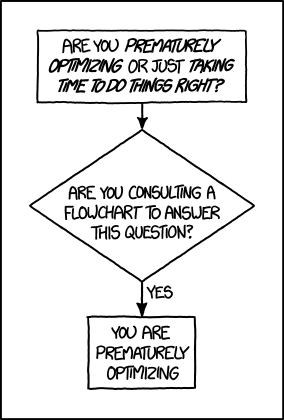
\includegraphics[height=\textheight]{optimization.png}
    
    {\tiny https://xkcd.com/1691/}
  \end{center}
  
\end{frame}

\begin{frame}[plain]
  \begin{center}
    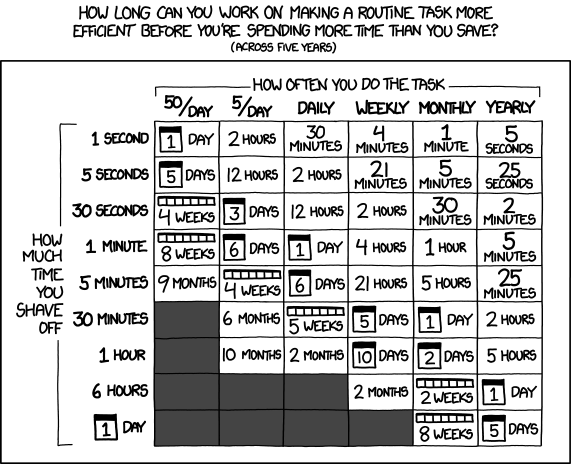
\includegraphics[height=\textheight]{is_it_worth_the_time.png}
    
    {\tiny https://xkcd.com/1205/}
  \end{center}
  
\end{frame}


\end{document}
%%% Local Variables:
%%% mode: latex
%%% TeX-master: t
%%% TeX-command-extra-options: "-shell-escape"
%%% End:
